
\hypertarget{thursday-january-9th}{%
\section{Thursday January 9th}\label{thursday-january-9th}}

\textbf{Recall:} For \(M^n\) a closed smooth manifold, consider a smooth
map \(f: M^n \to \RR\).

\textbf{Definition:} A critical point \(p\) of \(f\) is
\emph{non-degenerate} iff
\(\det( H\coloneqq \frac{\partial^i f}{\partial x_i \partial x_j}(p)) \neq 0\) in
some coordinate system \(U\).

\textbf{Lemma (The Morse Lemma)}: For any non-degenerate critical point
\(p\) there exists a coordinate system around \(p\) such that

\begin{align*}
f(x_1, \cdots, x_n) = f(p) - x_1^2 - x_2^2 - \cdots - x_\lambda^2 + x_{\lambda+1}^2 + \cdots + x_n^2
.\end{align*}

\(\lambda\) is called the \emph{index of \(f\) at \(p\)}.

\textbf{Lemma:} \(\lambda\) is equal to the number of \emph{negative}
eigenvalues of \(H(p)\).

\emph{Proof:} A change of coordinates sends \(H(p) \to A^t H(p) A\),
which (exercise) has the same number of positive and negative values.

\begin{quote}
Exercise: show this assuming that \(A\) is invertible and not
necessarily orthogonal. Use the fact that \(A^t H A\) is diagonalizable.
\end{quote}

This means that \(f\) can be written as the quadratic form

\begin{align*}
\left[\begin{array}{ccccc}
-2  & 0  & 0       & 0    & 0 \\
0   & -2 & 0       & 0    & 0 \\
0   & 0  & \ddots  &  0   & 0 \\
0   & 0  & 0       &  2   & 0 \\
0   & 0  & 0       &  0   & 2
\end{array}\right]
.\end{align*}

\emph{Proof of Morse Lemma:}

Suppose that we have a coordinate chart \(U\) around \(p\) such that
\(p\mapsto 0\in U\) and \(f(p) = 0\).

\textbf{Step 1 -- Claim:} There exists a coordinate system around \(p\)
such that

\begin{align*}
f(x) = \sum_{i,j=1}^n x_i x_j h_{ij}(x)
,\end{align*}

where \(h_{ij}(x) = h_{ji}(x)\).

\emph{Proof:} Pick a convex neighborhood \(V\) of \(0\in \RR^n\).

\begin{center}
    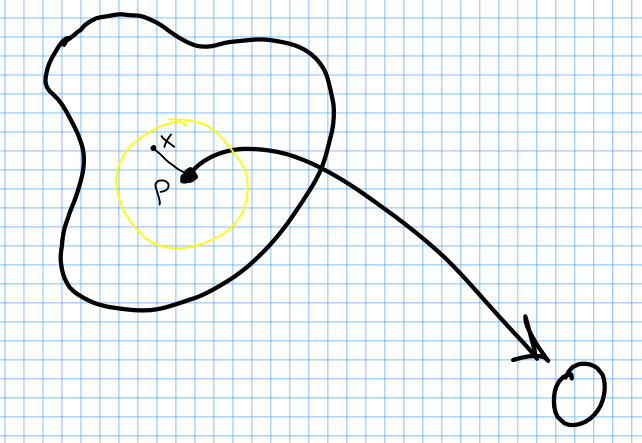
\includegraphics[width=\textwidth,keepaspectratio]{sections/figures/2020-01-09-11:38.png}\\
\end{center}


Restrict \(f\) to a path between \(x\) and \(0\), and by the FTC compute

\begin{align*}
I = \int_0^1 \frac{df(tx_1, tx_2, \cdots, tx_n) }{dt}  ~dt = f(x_1, \cdots, x_n) - f(0) = f(x_1, \cdots, x_n)
.\end{align*}

since \(f(0) = 0\).

We can compute this in a second way, \begin{align*}
I = \int_0^1 \dd{f}{x_1} x_1 + \dd{f}{x_2} x_2 + \cdots \dd{f}{x_n} x_n ~dt 
\implies \sum_{i=1}^n x_i \int_0^1  \dd{f}{x_i} ~dt = f(x)
.\end{align*}

We thus have \(f(x) = \sum_{i=1}^n x_i g_i(x)\) where
\(\dd{f}{x_i}(0) = 0\), and
\(\dd{f}{x_i} = x_1 \dd{g_1}{x_i} + \cdots + g_i + x_i \dd{g_i}{x_i} + \cdots + x_n \dd{g_n}{x_i}\).

When we plug \(x = 0\) into this expression, the only term that doesn't
vanish is \(g_i\), and thus \(\dd{f}{x_i}(0) = g_i(0)\) and
\(g_i(0) = 0\).

Applying the same result to \(g_i\), we obtain
\(g_i(x) = \sum_{j=1}^n x_j h_{ij}(x)\), and thus
\(f(x) = \sum_{i, j =1}^n x_i x_j h_{ij}(x)\).

We still need to show \(h\) is symmetric. For every pair \(i, j\), there
is a term of the form \(x_i x_j h_{ij} + x_j x_i h_{ji}\). So let
\(H_{ij}(x) = \frac{h_{ij}(x) + h_{ji}(x)}{2}\) (i.e.~symmetrize/average
\(h\)), then \(f(x) = \sum_{i, j = 1}^n x_i x_j H_{ij}(x)\) and this
shows claim 1.

\(\qed\)

\textbf{Step 2 -- Induction:} Assume that in some coordinate system
\(U_0\),

\begin{align*}
f(y_1, \cdots, y_n) = \pm y_1^2 \pm y_2^2 \pm \cdots \pm y_{r-1}^2 + \sum_{i, j \geq r} y_i y_j H_{ij}(y_1, \cdots, y_n)
.\end{align*}

Note that \(H_{rr}(0)\) is given by the top-left block of \(H_{ij}(0)\),
which is thus looks like

\begin{center}
   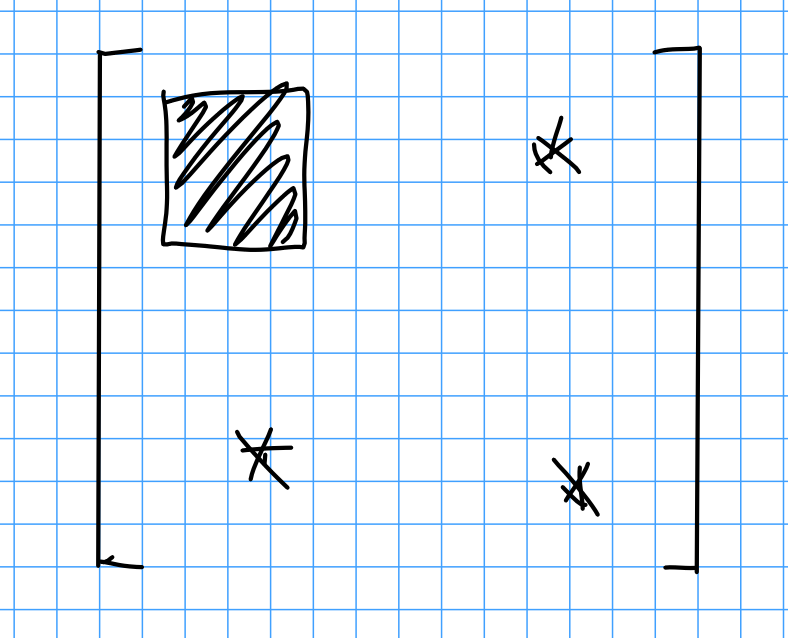
\includegraphics[width=0.25\textwidth,keepaspectratio]{sections/figures/2020-01-09-11:41.png}\\ 
\end{center}


Note that this block is symmetric.

Claim 1: There exists a linear change of coordinates such that
\(H_{rr}(0) \neq 0\).

We can use the fact that
\(\frac{\partial^2 f}{\partial x_i \partial x_j} (0) = H_{ij}(0) + H_{ji}(0) = 2 H_{ij}(0)\),
and thus
\(H_{ij}(0) = \frac{1}{2} \left( \frac{\partial f}{\partial x_i \partial x_j} \right)\).

Since \(H(0)\) is non-singular, we can find \(A\) such that
\(A^t H(0) A\) has nonzero \(rr\) entry, namely by letting the first
column of \(A\) be an eigenvector of \(H(0)\), then
\(A = [\vector v, \cdots]\) and thus
\(H(0)A = [\lambda \vector v, \cdots]\) and
\(A^t[\lambda \vector v] = [\lambda \norm{\vector v}^2, \cdots ]\).

So

\begin{align*}
&\sum_{i,j\geq r} y_i y_j H_{ij}(y_1, \cdots, y_n) \\
&= y_r^2 H_{rr}(y_1, \cdots, y_n) + \sum_{i > r} 2y_i y_r H_{ir}(y_1, \cdots, y_n) \\
&= H_{rr}(y_1, \cdots, y_n) \left( 
y_r^2 + \sum_{i > r} 2y_i y_r H_{ir}(y_1, \cdots, y_n)/H_{rr}(y_1, \cdots, y_n)
\right) \\
&= H_{rr}(y_1, \cdots, y_n) \left(
\left( y_r + \sum_{i > r}^n y_i H_{ir}(y_1, \cdots, y_n) / )_{rr}(y_1, \cdots, y_n) \right)^2
\sum_{i > r}^n y_i^2 \left( H_{ir}Y/H_{rr}(Y) \right)^2
\sum_{i, j > r}^n H_{ir}(Y)H_{jr}(Y)/H_{rr}(Y)
\right)^2 \quad\text{by completing the square}
.\end{align*}

\begin{quote}
Note that \(H_{rr}(0) \neq 0\) implies that \(H_{rr} \neq 0\) in a
neighborhood of zero as well.
\end{quote}

Now define a change of coordinates \(\phi: U \to \RR^n\) by
\begin{align*}
z_i = \begin{cases}
y_i & i\neq r \\
\sqrt{ H_{rr}(y_1, \cdots, y_n) } \left( y_r + \sum_{i> r} y_i H_{ir}(Y)/H_{rr}(Y) \right) & i=r
\end{cases}
.\end{align*}

This means that
\(f(z) = \pm z_1^2 \pm \cdots \pm z_{r-1}^2 \pm z_r^2 + \sum_{i, j \geq r+1^n z_i z_j \tilde{H}(z_1, \cdots, z_n) }\).

\begin{quote}
Exercise: show that \(d_0\phi\) is invertible, and by the inverse
function theorem, conclude that there is a neighborhood
\(U_2 \subset U_1\) of 0 on which \(\phi\) is still invertible.
\end{quote}

\(\qed\)

\textbf{Corollary:} The nondegenerate critical points of a Morse
function \(f\) are isolated.

\emph{Proof:} In some neighborhood around \(p\), we have
\(f(x) = f(p) - x_1^2 - \cdots - x_\lambda^2 + x_{\lambda + 1}^2 + \cdots + x_n^2\),
Thus \(\dd{f}{x_i} = 2x_i\), and so \(\dd{f}{x_i} = 0\) iff
\(x_1 = x_2 = \cdots = x_n = 0\).

\textbf{Corollary:} On a closed (compact) manifold \(M\), a Morse
function has only finitely many critical points.

We will need these facts to discuss the \(h\dash\)cobordism theorem. For
a closed smooth manifold, \(\partial M = \emptyset\), so \(M\) will define a
cobordism \(\emptyset \to \emptyset\).

\textbf{Definition:} Let \(W\) be a cobordism from \(M_0 \to M_1\). A
\emph{Morse function} is a smooth map \(f: W\to [a, b]\) such that

\begin{enumerate}
\def\labelenumi{\arabic{enumi}.}
\tightlist
\item
  \(f\inv(a) = M_0\) and \(f\inv(b) = M_1\),
\item
  All critical points of \(f\) are non-degenerate and contained in
  \(\mathrm{int}(W) \definedas W\setminus \partial W\).
\end{enumerate}

\begin{quote}
So \(f\) is equal to the endpoints only on the boundary.
\end{quote}

\begin{quote}
Next time: existence of Morse functions. This is a fairly restrictive
notion, but they are dense in the \(C^2\) topology on (?).
\end{quote}
